\RequirePackage{shellesc}
\immediate\write18{cd ..; tex braids_code.dtx}

\documentclass{article}

\usepackage{tikz}
\usetikzlibrary{braids}

\begin{document}
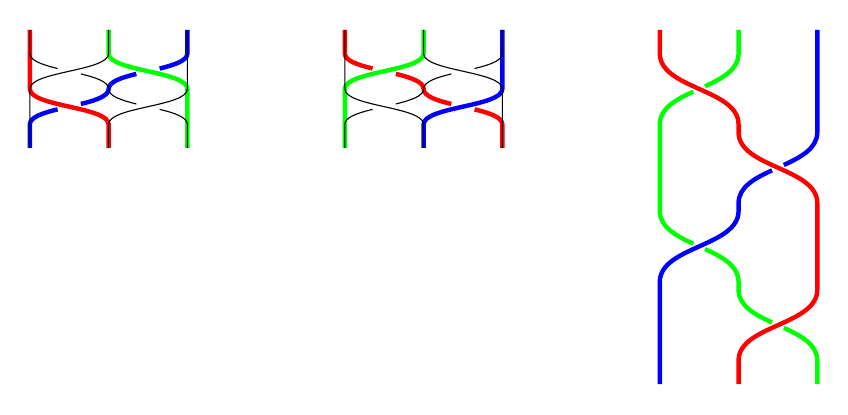
\begin{tikzpicture}
\pic[
  braid/.cd,
  strand 1/.style={red,ultra thick},
  strand 2/.style={green,ultra thick},
  strand 3/.style={blue,ultra thick}
] {braid={s_{1-3}}};
\pic[
  at={(4,0)},
  braid/.cd,
  strand 1/.style={red,ultra thick},
  strand 2/.style={green,ultra thick},
  strand 3/.style={blue,ultra thick}
] {braid={s_{3-1}}};
\begin{scope}%[yshift=-2cm]
\pic[
  braid/.cd,
%  strand 1/.style={red,ultra thick},
%  strand 2/.style={green,ultra thick},
%  strand 3/.style={blue,ultra thick}
] {braid={s_{1-3}^{-1}}};
\pic[
  at={(4,0)},
  braid/.cd,
%  strand 1/.style={red,ultra thick},
%  strand 2/.style={green,ultra thick},
%  strand 3/.style={blue,ultra thick}
] {braid={s_{3-1}^{-1}}};
\end{scope}

\pic[
  at={(8,0)},
  braid/.cd,
  strand 1/.style={red,ultra thick},
  strand 2/.style={green,ultra thick},
  strand 3/.style={blue,ultra thick}
] {braid={s_1 s_2 s_1^{-1} s_2^{-1}}};
\end{tikzpicture}
\end{document}
